\documentclass[12pt, a4paper]{article}
\usepackage[french]{babel}
\usepackage{caption}
\usepackage{graphicx}
\usepackage[T1]{fontenc}
\usepackage{listings}
\usepackage{geometry}
\usepackage{wrapfig}
\usepackage{mwe}

\usepackage[toc,page,header]{appendix}
\usepackage{minitoc}
\usepackage[backref=page,plainpages=false,pdfpagelabels,colorlinks=true,linkcolor=black,anchorcolor=black,citecolor=black,filecolor=black,menucolor=black,runcolor=black,urlcolor=black]{hyperref}


\usepackage{ragged2e}
\usepackage[table, dvipsnames]{xcolor}
\usepackage[style=listgroup,acronym,toc]{glossaries}

\setglossarystyle{long}

\newacronymstyle{ex-footnote}%
{%
  \GlsUseAcrEntryDispStyle{footnote}%
}%
{%
  \GlsUseAcrStyleDefs{footnote}%
  \renewcommand*{\genacrfullformat}[2]{%
   \firstacronymfont{\glsentryshort{##1}}##2%
   \expandafter\footnote\expandafter{\expandafter\glsentrylong\expandafter{##1}}%
  }%
  \renewcommand*{\Genacrfullformat}[2]{%
   \firstacronymfont{\Glsentryshort{##1}}##2%
   \expandafter\footnote\expandafter{\expandafter\glsentrylong\expandafter{##1}}%
  }%
  \renewcommand*{\genplacrfullformat}[2]{%
   \firstacronymfont{\glsentryshortpl{##1}}##2%
   \expandafter\footnote\expandafter{\expandafter\glsentrylongpl\expandafter{##1}}%
  }%
  \renewcommand*{\Genplacrfullformat}[2]{%
   \firstacronymfont{\Glsentryshortpl{##1}}##2%
   \expandafter\footnote\expandafter{\expandafter\glsentrylongpl\expandafter{##1}}%
  }%
}

\setacronymstyle{ex-footnote}
\makeglossaries
 
\newacronym{UCI}{UCI}{Unité Client Intervention}
\newacronym{FTTH}{FTTH}{Fiber To The Home}
\newacronym{D2}{D2}{Réseau de distribution entre le PM et PB}
\newacronym{PM}{PM}{Point de Mutualisation}
\newacronym{PB}{PB}{Point de Branchement}
\newacronym{PTO}{PTO}{Prise Terminale Optique}
\newacronym{OB}{OB}{Orange Business}
\newacronym{GP}{GP}{Grand Public}
\newacronym{SAV}{SAV}{Service Après Vente}
\newacronym{PMI}{PMI}{Point de Mutualisation Immeuble}
\newacronym{PMZ}{PMZ}{Point de Mutualisation de Zone de 360 logements}
\newacronym{OPO}{OPO}{Optimal Pro Office}
\newacronym{PMS}{PMS}{Dérangement prélocalisé multiservices}
\newacronym{ROI}{ROI}{FTTH retour Opérateur Infrastructure}
\newacronym{EXP}{EXP}{Expertise}







\usepackage{xcolor}
\definecolor{codeviolet}{rgb}{0.3,0.0,0.3}
\definecolor{codegray}{rgb}{0.5,0.5,0.5}
\definecolor{codepurple}{rgb}{0.58,0,0.82}
\definecolor{backcolour}{rgb}{0.93,0.93,0.93}

\lstdefinestyle{mystyle}{
    backgroundcolor=\color{backcolour},   
    commentstyle=\color{codeviolet},
    keywordstyle=\color{magenta},
    numberstyle=\tiny\color{codegray},
    stringstyle=\color{codepurple},
    basicstyle=\ttfamily\footnotesize,
    breakatwhitespace=false,         
    breaklines=true,                 
    captionpos=b,                    
    keepspaces=true,                 
    numbers=left,                    
    numbersep=5pt,                  
    showspaces=false,                
    showstringspaces=false,
    showtabs=false,                  
    tabsize=2
}

\usepackage{graphicx, wrapfig, calc}
\input{insbox}
\usepackage{lipsum}


\usepackage[edges]{forest}
\forestset{
  direction switch/.style={
    for tree={edge+=thick},
    where level>=1{folder, grow'=0}{for children=forked edge},
    where level=3{}{draw},
  },
}

\geometry{
  left=2.5cm,
  right=2.5cm,
  top=2.5cm,
  bottom=2.5cm,
}
\usepackage{pgfplots}



\usepackage{xcolor}
\usepackage{xcolor,rotating,epic,eepic}
\usepackage{tikz-qtree}
\usetikzlibrary{matrix}

\usepackage{xcolor,rotating,epic,eepic}
\usepackage{tikz}
\usepackage[babel=true,kerning=true]{microtype}


\usepgfplotslibrary{polar}
\pgfplotsset{compat=1.12} 

\newenvironment*{remerciements}{%
\renewcommand*{\abstractname}{Remerciements}
\begin{abstract}
}{\end{abstract}}

\pgfplotsset{width=10cm,compat=1.9}
\usepackage{fancyhdr}
\pagestyle{fancy}
\lhead{}
\rhead{}
\chead{}
\rfoot{\thepage}
\lfoot{}
\cfoot{}


\renewcommand{\headrulewidth}{0.4pt}
% \renewcommand{\footrulewidth}{0.4pt}

\begin{document}
\begin{titlepage}
	\newcommand{\HRule}{\rule{\linewidth}{0.5mm}} 
	\center 
	\textsc{\LARGE iut de colmar}\\[6.5cm] 
	
	\textsc{\Large département réseaux et télécommunications}\\[0.5cm] 
	\textsc{\large en alternance chez orange}\\[0.5cm]
	\HRule\\[0.75cm]
	{\Large\bfseries Connectivité et Innovation : Mon Parcours d'Alternance au sein d'Orange}\\[0.4cm]
	\HRule\\[0.5cm]
	\textsc{\large candidat : martin baumgaertner\\
	tuteur universitaire : m. albert\\
	maître de stage : m. camille }\\[5cm] 
	\begin{figure}[h]
		\centering
		
\includegraphics[width=0.5\textwidth]{img/uha.png}
	\end{figure}
	\begin{figure}[h]
		\centering
		
\includegraphics[width=0.1\textwidth]{img/orange.png}
	\end{figure}

	\vfill\vfill\vfill
	% {\large\today} 
	\vfill
\end{titlepage}
\newpage
\pagestyle{empty}
\begin{remerciements}
	\textit{Je tiens à exprimer ma sincère gratitude envers toute l'équipe d'Orange chez 
	laquelle j'ai eu le privilège de réaliser mon alternance. Mes remerciements
	vont particulièrement à Félix Camille et Osman Demir, qui m'ont guidé tout
	au long de cette expérience enrichissante.}\\

	\textit{Je tiens également à remercier l'ensemble de mes collègues pour leur accueil
	chaleureux et leur collaboration précieuse. Leur expertise et leur soutien ont
	grandement contribué à mon apprentissage et à mon développement professionnel.}\\

	\textit{Enfin, je souhaite exprimer ma reconnaissance envers l'équipe pédagogique de
	l'IUT de Colmar pour leur accompagnement et leur suivi tout au
	long de cette alternance.}\\

	\textit{Merci à tous ceux qui ont rendu cette expérience aussi mémorable que formatrice.}
	
\end{remerciements}
\newpage
\doparttoc
\tableofcontents
\newpage
\listoffigures
\newpage
\part{\Large{Rapport}}
\newpage
\pagestyle{fancy}
\section{Préambule}
Je suis ravi de présenter ce rapport, fruit de mon expérience en alternance chez Orange.\\

Orange est un leader mondial dans les télécommunications et les services mobiles.
L'entreprise, engagée dans l'innovation et la connectivité, joue un rôle majeur dans la
transformation numérique en offrant des solutions variées aux particuliers et aux entreprises.\\

En tant qu'acteur évoluant au sein de la nouvelle
stratégie d'Orange baptisée "Lead The Future",
je m'identifie particulièrement au premier axe
qui consiste à \textit{valoriser notre cœur de métier pour
renforcer notre excellence et notre qualité de
service}. En tant que leader du déploiement de la
fibre optique en Europe avec 46 millions de prises
FTTH déployées fin 2022,
Orange détient une base d'actifs technologiques
considérables. L'accent mis sur l'excellence du
réseau, résultat d'investissements massifs,
renforcera notre position de leader en matière
d'expérience client. Enfin,
en se tournant résolument vers les usages
de demain, "Lead The Future" capitalisera sur
l'expertise de ses chercheurs et collaborateurs
dédiés à l'innovation, en construisant des services
et usages novateurs tels que les réseaux
d'entreprises à la demande et le WiFi du futur à
la maison.

Pendant mon alternance, j'ai travaillé au sein du département \gls{UCI} EST.
En tant que technicien d'invervention grand public, j'ai contribué aux projets de l'équipe, collaboré avec des
professionnels et développé une compréhension des défis et des opportunités
de cette entreprise.\\


L'engagement d'Orange envers l'excellence et l'innovation a profondément influencé ma vision
professionnelle. Ce rapport vise à refléter et à analyser les enseignements tirés de cette
expérience, mettant en lumière les aspects les plus pertinents de mon parcours au sein de
cette entreprise emblématique.\\

Tout au long de mon alternance j'ai pu réaliser différentes missions
toutes plus importantes les unes que les autres. J'ai travaillé sur des projets
d'envergure, et j'ai pu découvrir le monde de l'entreprise.
Je m'occupais principalement d'installations d'offres
Connect Pro, la prestation "installation experte", 
de contrôles de qualité d'installation et de dépannages.\\


Au cours de ce rapport, je vais détailler les différentes facettes de mon expérience,
en commençant par une rétrospective de l'histoire d'Orange, suivie d'une exploration
approfondie du département UCI EST et des missions cruciales auxquelles
j'ai participé.\\
Après avoir présenté ce contexte, je partagerai une analyse approfondie
de mon expérience, en mettant en évidence les enseignements tirés,
les compétences développées et les différentes corrélations 
que je peux faire avec le B.U.T. Cette réflexion sera étayée par des exemples
concrets de missions spécifiques, illustrant ainsi la manière dont mon
alternance chez Orange a façonné mon expérience professionnelle.\\
Le rapport se terminera par une synthèse de mes contributions à
l'innovation et à la stratégie globale d'Orange, ainsi que par un
bilan personnel où je partagerai mes réflexions sur cette expérience
enrichissante et les perspectives qu'elle ouvre pour l'avenir.\\
Ainsi, ce rapport sera une plongée détaillée dans mon parcours
d'alternance chez Orange.


\newpage
\section{Présentation de l'entreprise}
\subsection{Historique}
L'histoire d'Orange est emblématique en France, ayant évolué au gré des
innovations technologiques et des réformes structurelles. Originellement connue
sous le nom des PTT (Postes, Télégraphes et Téléphones), 
l'entreprise a été le pilier des services de communication en
France. En 1990, les PTT ont été divisés en deux entités distinctes : La Poste et France Télécom.
C'est d'ailleurs pour cette raison que partout en France, les bureaux de postes 
sont très souvent situés à côtés de centraux téléphoniques d'Orange.\\

A la date du 1er juillet 2013, France Télécom deviendra Orange, et ce dans le monde entier.
Ainsi, nous pouvons retrouver Orange dans pas moins de 26 pays à travers le monde et 
compte près de plus de 140 000 collaborateurs.\\

Le siège social d'Orange est situé à Issy-les-Moulineaux,
et est dirigé par Christel Heydemann. Pour ma part, 
j'ai effectué mon alternance en étant rattaché 
à l'agence de Schiltigheim. Nous pouvons retrouver 
dans ces bureaux de nombreux collaborateurs et 
plusieurs équipes, notamment des chargés d'affaires
et des techniciens d'intervention. Au sein de l'UCI EST,
nous retrouvons plusieurs équipes d'interventions :\\

\textbf{A REVOIR}\\

\begin{itemize}
	\item Equipe d'invervention sur le réseau structurant 
	\item Equipe d'intervention entreprise
	\item Equipe d'intervention grand public\\
\end{itemize}

Pour ma part, j'ai effectué mon alternance en tant que
technicien d'intervention grand public dans l'équipe
d'Osman Demir. 


\subsection{Mon service}
Comme décrit précédemment, mon alternance s'est déroulée
dans l'équipe d'intervention grand public 
du bas-rhin. Nous sommes amenés à réaliser des missions diverses et 
variées, comme des 
expertises, des installations, des dépannages et 
des contrôles de qualité.\\

Le but d'une expertise \gls{FTTH} est de se rendre chez un client
qui a déjà eu plusieurs rendez-vous \gls{SAV} et qui n'a pas eu de solution. 
Notre objectif est alors d'en apporter une et que l'on 
soit le dernier technicien à se rendre chez le client.\\

Les installations que nous sommes amenés à réaliser sont
la mise en service de l'offre Connect Pro d'Orange et 
la prestation installation experte (qui seront détaillées dans les parties suivante)
en plus de toutes les prestations sur le réseau cuivre.\\


\begin{figure}
	\centering
	\begin{forest}
		direction switch
		[\textbf{Directrice Générale - Christel Heydemann}
		[CEO Orange France - \textbf{Jean François Fallacher}
			[Directeur Grand Ouest]
			[...]
			[Directeur Grand Nord Est - \textbf{Thierry Marigny}
			[Directeur distribution Orange Est]
			[...]
			[Directeur Unité Intervention Est - \textbf{Jean Luc Aribaud}
			[Directeur Appui Intervention et Pilotage Clients]
			[...]
			[Directeur Intervention et Réseau Alsace - \textbf{Thomas Mall}
			[Responsable d'équipe - \textbf{Patricia Babula}]
			[Responsable CSC de Mulhouse - \textbf{Sandra Nadeau}
			[Thomas Strub]
			[...]
			]
			[Responsable Opérateur Commercial Réseau Alsace - \textbf{Aurore Kimenau}
			[Louis Pluviose]
			[...]
			]
			[Responsable Opérateur Commercial Service Alsace - \textbf{Osman Demir}
			[\textbf{Martin Baumgaertner}]
			[Julien Losser]
			[Felix Camille]
			[...]
			]
			]
			]
			]
		]
		[CEO Orange Cyberdéfense
		[...
		]
		]
		[...]
		]
	\end{forest}
	\caption{Organigramme simplifié d'Orange}
\end{figure}

\newpage
Nous pouvons voir ci-dessus un organigramme 
très simplifié d'Orange. Le but est de montrer
ma position dans l'entreprise. Nous pouvons alors
voir toute la hiérarchie. Je n'ai pas mis tous les 
noms des techniciens dans mon équipe mais seulement 
les personnes citées dans le rapport et mes collègues 
de promotion. Au total 60?? techniciens dans 
l'équipe d'Osman Demir. 

\newpage 
\section{Mes missions}
\subsection{Introduction}
Au cours de mon alternance de 2 ans. J'ai eu la chance
de pouvoir effectuer des missions riches en 
enseignements, avec toujours des cas différents. 
Ma première année s'est déroulée en doublure avec 
mon tuteur Félix. Il m'a fait monter en compétences
et m'a permis de découvrir le monde de l'entreprise.
C'est grâce à lui que j'ai pu acquérir le
nécessaires pour être autonome. Suite à cette première
année, j'ai pu réaliser des missions seul, qui ont aussi 
été très enrichissantes. Car même si Félix m'a appris 
beaucoup de choses, il y a toujours des cas complexes 
sur lesquels nous n'étions jamais tombé en 1 an et
qui nécessitent de la réflexion. Grâce à son soutien 
téléphonique en cas de besoin, j'ai pu alors
devenir de plus en plus autonome. Toutes les missions 
que je vais présenter ci-après sont ma vie professionnelle
de tous les jours. Il n'y aura qu'une seule mission 
ponctuelle que j'ai effectué pendant 4 jours que je 
vous présenterai en dernière partie.

\subsection{Ma première installation}
A mon arrivée dans l'équipe, et mes débuts chez Orange, 
je me rappelerai toujours de ma première installation 
avec Félix. C'était dans une mairie dans le nord
de l'Alsace qui avait la particularité d'avoir 
souscrit à 2 offres Connect Pro (pour deux services différents) 
alors qu'ils étaient dans les mêmes locaux. Je me rappelle que Félix m'avait
montré comment faire la première puis, il m'avait laissé
faire la seconde. Assez facile me direz-vous, mais
c'était sans compter sur le stress de découvrir 
une nouvelle solution, avec un process que je ne connaissais 
pas. C'était les débuts de l'apprentissage. 

\subsection{Connect Pro}
\subsubsection{Présentation}
Connect Pro d'Orange représente une solution
de téléphonie IP novatrice, spécialement conçue pour
les petites entreprises. Elle offre la flexibilité et
la facilité d'utilisation dont ces entreprises ont
besoin pour gérer leurs communications de manière
efficace, sans la nécessité d'investir dans un
serveur IPBX physique sur site. Tout est géré de
manière transparente dans le cloud, grâce aux
serveurs d'Orange, à partir de la Livebox
que nous installons.\\

Ce qui distingue cette offre, c'est sa
personnalisation approfondie. Les clients ont
la possibilité de créer des messages personnalisés 
fait par un studio d'enregistrement professionnel 
pour accueillir leurs appelants; des prédécrochés
informatifs, des messages d'attente professionnels
et des répondeurs adaptés à leurs besoins spécifiques.
Cela leurs permet de fournir une expérience de
communication personnalisée à leurs clients
et partenaires.\\

Mais ce n'est pas tout, car la personnalisation
va encore plus loin. Par exemple, nous
pouvons paramétrer un envoi automatique de
mails à chaque fois qu'un message est déposé sur
le répondeur. Ces mails peuvent contenir le
message vocal en pièce jointe, ce qui
facilite la gestion et le suivi des messages importants.\\

\newpage
\begingroup
\setlength{\intextsep}{0pt}
\begin{wrapfigure}[20]{R}{6.5cm}
	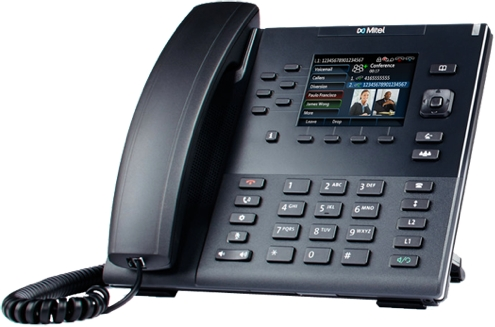
\includegraphics[scale=.5]{img/mittel.jpg}
	\caption{Poste Mittel 67i \cite{r1}}
\end{wrapfigure}
De plus, Connect Pro propose une variété
d'options en matière de téléphones, que
ce soit des téléphones sans fil pour
une mobilité accrue, des téléphones
filaires pour une utilisation plus
traditionnelle ou bien même des softphone 
sur PC ou smartphone disponibles avec 
l'application Cisco Webex. Cela signifie que nous pouvons
adapter la solution de téléphonie exactement aux besoins
des clients et à son environnement de travail.
Ci-contre nous pouvons observer un poste Mittel 67i
qui est un poste filaire, ainsi qu'un poste sans fil
Yealink W76P.\\
\begin{wrapfigure}[20]{R}{6.5cm}
	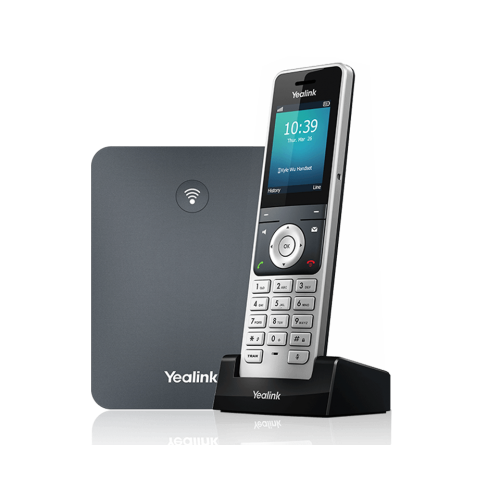
\includegraphics[scale=.6]{img/yealink.png}
	\caption{Yealink W76P \cite{r2}}
\end{wrapfigure}

Bien sûr, il est important de noter que l'offre
Connect Pro d'Orange propose une flexibilité en
fonction de la technologie d'accès disponible dans
la zone du client. Pour les entreprises situées dans des
zones couvertes par la fibre optique, l'offre
"Connect Pro Fibre" offre la possibilité de
bénéficier de jusqu'à 20 lignes téléphoniques.\\

Cependant, il est important de noter qu'il
existe également une version de l'offre Connect Pro
pour les entreprises situées dans des zones
couvertes par le cuivre : "Connect Pro Cuivre"
Cette solution est disponible dans ces régions, mais elle est
généralement limitée en termes de capacité et de
fonctionnalités par rapport à la version fibre.
En général, les entreprises optent pour
Connect Pro Cuivre uniquement lorsqu'elles ont
des besoins de communication très basiques, tels
que 1 ou 2 postes, car les réseaux
cuivre ne permettent pas une utilisation aussi
étendue ni des fonctionnalités aussi avancées 
que la fibre.\\

En fin de compte, le choix entre "Connect Pro
Fibre" et "Connect Pro Cuivre" dépendra de la
disponibilité de la technologie dans la région du client,
ainsi que de leurs besoins en matière de communication.
\par\endgroup

\newpage
\subsubsection{Installations Connect Pro}
Lors de l'installation d'offres Connect Pro, nous
avons un process à suivre. Tout d'abord, nous devons
vérifier le dossier client afin de s'assurer 
qu'il n'y ait pas d'erreurs. Nous contrôlons 
le numéro de téléphone, et surtout, les adresses 
MAC des postes téléphoniques. En effet, il est
important de vérifier ce paramètre car si elles 
sont erronées, les postes n'auront pas 
la bonne configuration.\\

Une fois la vérification effectuée, nous pouvons
commencer l'installation. Nous commençons généralement 
par installer la Livebox en important les différents 
paramètres de configuration personnalisé que le client 
aurait pu faire.\\

Ensuite, nous installons les postes téléphoniques
en les connectant en RJ45 à la Livebox. Une fois
les postes installés, nous pouvons alors les
configurer. Pour cela, nous nous rendons sur 
l'interface web suivante : \url{https://connect.pro.orange.fr/}
et nous nous connectons avec les identifiants
du client.\\

Nous arrivons alors sur l'interface de gestion
de l'offre Connect Pro : 
\begin{figure}[h]
	\centering
	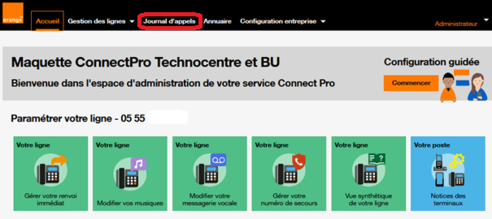
\includegraphics[scale=1.3]{img/accueil.png}
	\caption{Accueil de l'interface de gestion \cite{r3}}
\end{figure}

Nous retrouvons alors tous nos postes 
dans la partie "Gestion de lignes". Nous pouvons
les configurer selon les besoins de client. 

\begin{figure}[h]
	\centering
	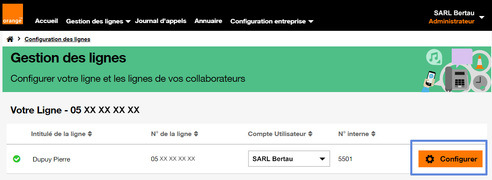
\includegraphics[scale=0.65]{img/configuration.jpg}
	\caption{Configuration des postes \cite{r4}}
\end{figure}

\newpage
\subsubsection{Tests et vérifications}
Une fois l'installation terminée, nous devons
vérifier que la programmation de la téléphonie 
soit correcte. Pour cela, il suffit de faire 
un appel entrant et s'assurer que les différents
messages, les renvois vers d'autres postes et
les répondeurs fonctionnent correctement. 
Nous nous assurons également qu'en cas 
de coupure de courant, tous les appels entrants
soient redirigés vers un numéro de secours.\\

Cette phase de tests est cruciale car elle permet 
de détecter les éventuelles erreurs ou anomalies
avant de présenter et de former le client 
à sa nouvelle solution de téléphonie.\\

\subsubsection{Difficultés rencontrées}
La plupart des difficultés rencontrées lors des installations
Connect Pro étaient liées aux équipements clients présents.
Parmi les principaux défis que j'ai dû surmonter,
trois se sont révélés particulièrement prépondérants. 
Comme le fait que certains câbles RJ45 étaient mal identifiés, ce qui a entraîné
des retards et des erreurs potentielles.\\

Dans certains cas, les installations présentaient un enchevêtrement
complexe de câbles, compliquant la compréhension du réseau.
J'essayais toujours de simplifier ces installations en retirant les câbles
inutiles et en ordonnant les câbles restants.\\

Mais aussi, il m'est arrivé plusieurs fois d'être face à de vieux bâtiments 
manquants drastiquement de prises électriques pour alimenter les équipements
nécessaires. Il fallait alors essayer de trouver des solutions 
provisoires, comme la mise en 
place d'enrouleurs multiprise le temps que le client fasse les travaux nécessaires. 

Malgré ces défis, une approche proactive et une communication efficace
avec les clients ont permis de mener à
bien les installations Connect Pro. Ces
expériences m'ont permis de développer des compétences essentielles
en résolution de problèmes tout en
renforçant ma capacité à travailler dans des environnements complexes.



\newpage
\subsubsection{Ma contribution à l'innovation}
Au cours de toutes les installations effectuées, 
je me suis souvent rendu compte que les clients
voulaient souvent mettre en place des messages 
de répondeur temporaire pour les périodes
de fermetures exceptionnelles. Cependant,
la méthode est souvent fastidieuse et
complexe pour les clients, et ils l'oublient 
souvent. C'est pourquoi j'ai eu l'idée de
créer une maquette explicative pour les clients
afin qu'ils gardent une trace de la procédure. 
La voici ci-dessous, et en grand format en annexe.\\
\begin{figure}[h]
	\centering
	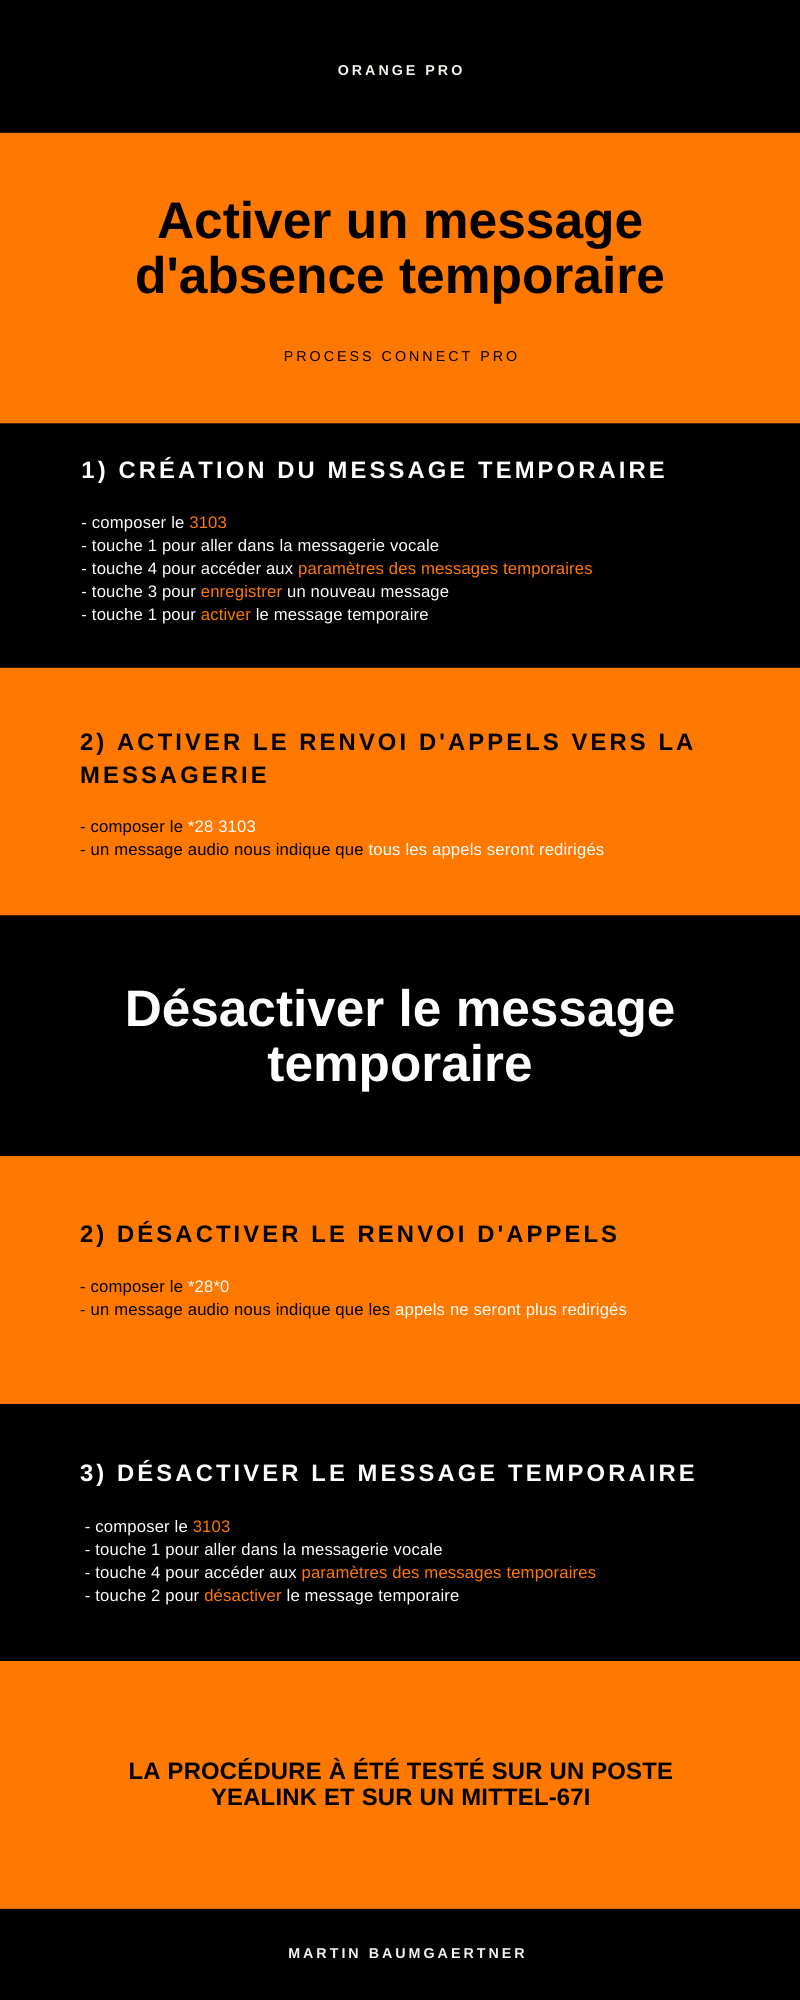
\includegraphics[scale=0.3]{img/maquette.png}
	\caption{Maquette explicative}
\end{figure}
\newpage

\subsubsection{Les similitudes avec l'IUT}
Lorsqu'au semestre 3 nous avons eu la SAE "Déployer un service de 
téléphonie multi-sites" avec M. Hensel, j'ai pu me rendre compte
que les installations Connect Pro étaient très similaires à ce que
nous avions fait pendant le projet et les TP. En effet, nous avions installé un serveur
Asterisk et des postes téléphoniques. Nous les avions configurés 
en ligne de commande. J'ai pu comprendre comment l'offre Connect Pro 
est géré en backend sur les serveurs d'Orange. Par exemple, 
nous avons parametrés en SAE un message de prédécroché,
un message d'attente et un message de répondeur. 
Pour le prédécroché, il fallait déclarer une nouvelle 
classe dans le fichier \texttt{musiconhold.conf} : 

\begin{lstlisting}[language=bash, style=mystyle]
[predec]
mode=files
directory=/var/lib/asterisk/sounds/mohpre
random=yes
\end{lstlisting}
Puis, il fallait ensuite dans le fichier \texttt{extensions.conf}
modifier le plan de numérotation afin d'associer le prédécroché
aux numéros des 3 postes que nous avions : 
\begin{lstlisting}[language=bash, style=mystyle]
exten => 1,2,Dial(PJSIP/TM1,3O,tTwWm(newclass))
exten => 2,2,Dial(PJSIP/TM1BIS,3O,tTwWm(newclass))
exten => 3,2,Dial(PJSIP/TL1,3O,tTwWm(newclass))
\end{lstlisting}

Toutes ces notions apprises en SAE m'ont permis de mieux comprendre
le fonctionnement de l'offre Connect Pro et de mieux appréhender
les installations. Comprendre que derrière un seul bouton 
à cliquer sur l'interface web, se cache 
en réalité une multitude de commandes envoyés sur le serveur
d'Orange.\\

Ainsi, cette expérience chez Orange a clairement illustré la manière
dont les compétences acquises au cours de ma formation ont pu être
mises en pratique dans le déploiement de services de téléphonie.
Cela a non seulement renforcé ma compréhension des
concepts théoriques, mais m'a également permis de les appliquer
dans un contexte professionnel concret. Cette convergence entre
la théorie et la pratique a enrichi ma formation et a contribué
à façonner ma croissance professionnelle.

\newpage
\subsection{Installation experte}
\subsubsection{Présentation}
L'installation experte d'Orange est une
prestation payante en option qui offre aux clients
une prise en charge complète de l'installation de leurs
équipements Orange, notamment la Livebox, le/les décodeur(s)
et les répéteurs si nécessaire. Cette offre vise à simplifier
l'expérience des clients en garantissant une configuration
correcte et en optimisant la performance de leurs équipements.\\

L'un des aspects essentiels de cette prestation est la
connexion de tous les équipements clients au réseau Wi-Fi.
Nous nous assurons que chaque appareil est
correctement connecté et qu'il bénéficie d'une connexion
stable et sécurisée à Internet. De plus, en fonction des besoins
spécifiques du client, nous personnalisons les paramètres Wi-Fi
pour répondre aux exigences particulières, garantissant ainsi
une expérience Internet adaptée à chaque foyer.\\

De plus, l'installation experte comprend également une analyse
complète de la couverture Wi-Fi en fonction des différentes
pièces de la maison du client. Nous évaluons
la qualité du signal dans chaque zone et proposons des
suggestions d'installation de répéteurs si nécessaire. Cette
démarche a pour objectif d'optimiser la portée du signal Wi-Fi,
d'éliminer les zones mortes et de garantir une connectivité fluide
dans l'ensemble de l'espace couvert.
\subsubsection{La prestation installation experte}
Plusieurs étapes essentielles sont nécessaires pour garantir
la réussite d'une installation experte, chacune contribuant à offrir
une expérience optimale au client. La première étape consiste à
effectuer une vérification du dossier client, en examinant notamment
si les positions au \gls{PM} sont clairement indiquées.
Lorsque ces informations sont disponibles, nous nous rendons
directement au point de mutualisation, où nous procédons à la
mise en place d'une jarretière optique. Cette étape permet d'établir
la connexion du client au réseau Orange.\\

Cependant, dans le cas où les positions au point de mutualisation ne
sont pas préalablement renseignées, une autre démarche s'impose.
Nous devons alors nous diriger vers le \gls{PB}
pour identifier la couleur du tube et de la fibre client.
Cette opération est réalisée à l'aide d'un laser émis depuis
la \gls{PTO}, permettant ainsi d'obtenir les
informations nécessaires. Une fois en possession de ces données,
nous sollicitons un service spécialisé, "l'appui à chaud". Cette
équipe dédiée est en mesure de nous fournir la position exacte du
client du côté client, facilitant ainsi la connexion au réseau Orange.\\

\newpage
Ci-après, nous pouvons observer deux types de points de branchement
différents. Le premier situé en chambre. Tandis que le deuxième est un \gls{PB} que l'on peut
rencontrer est positionné sur un poteau, principalement dans les zones où
les câblages sont aériens.
\begin{figure}[htbp]
    \centering
    \begin{minipage}[b]{0.4\textwidth}
		{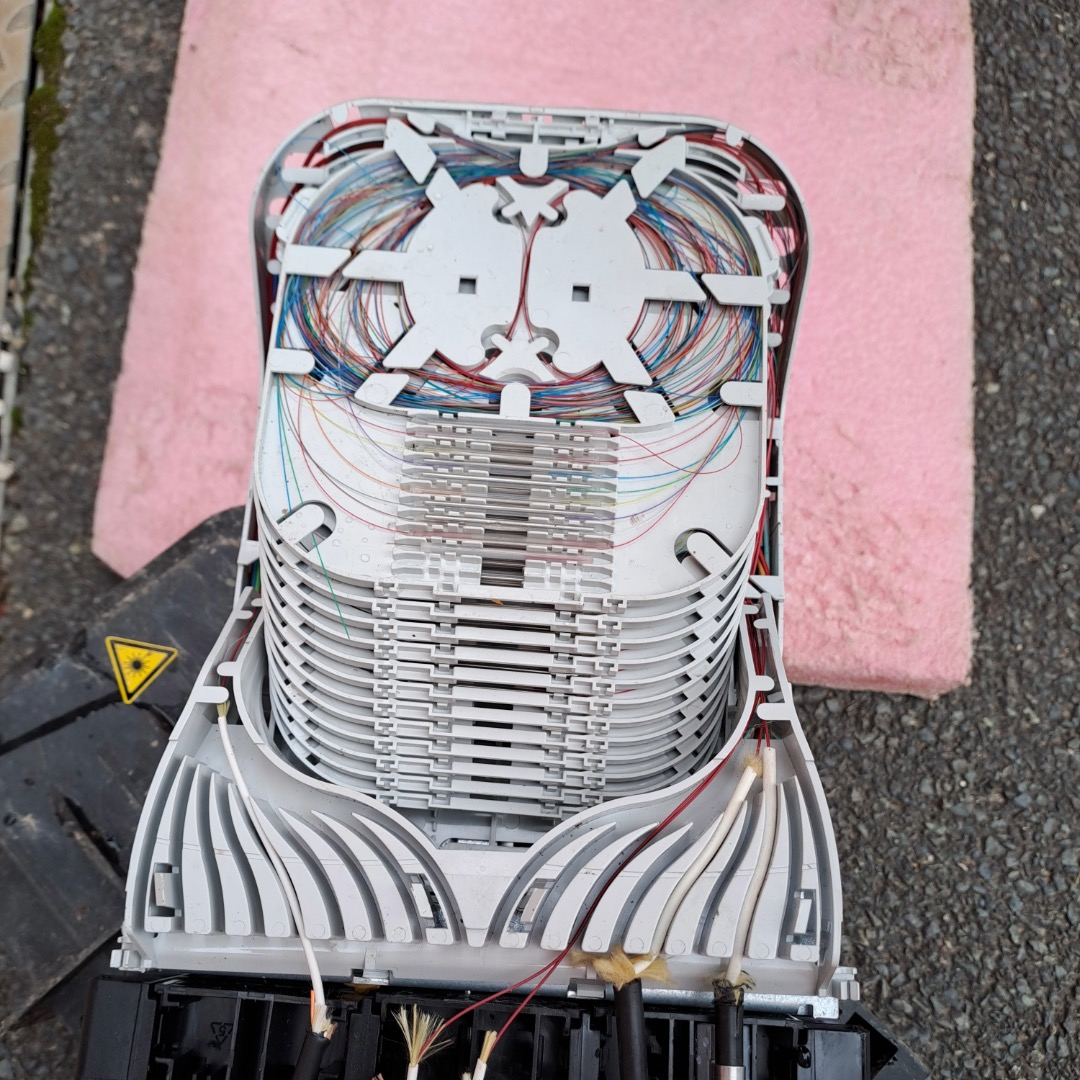
\includegraphics[width=\textwidth]{img/pbc.jpg}}
      \caption{PB en chambre}
    \end{minipage}
    \hspace{0.5cm} % Espace horizontal entre les deux images
    \begin{minipage}[b]{0.4\textwidth}
      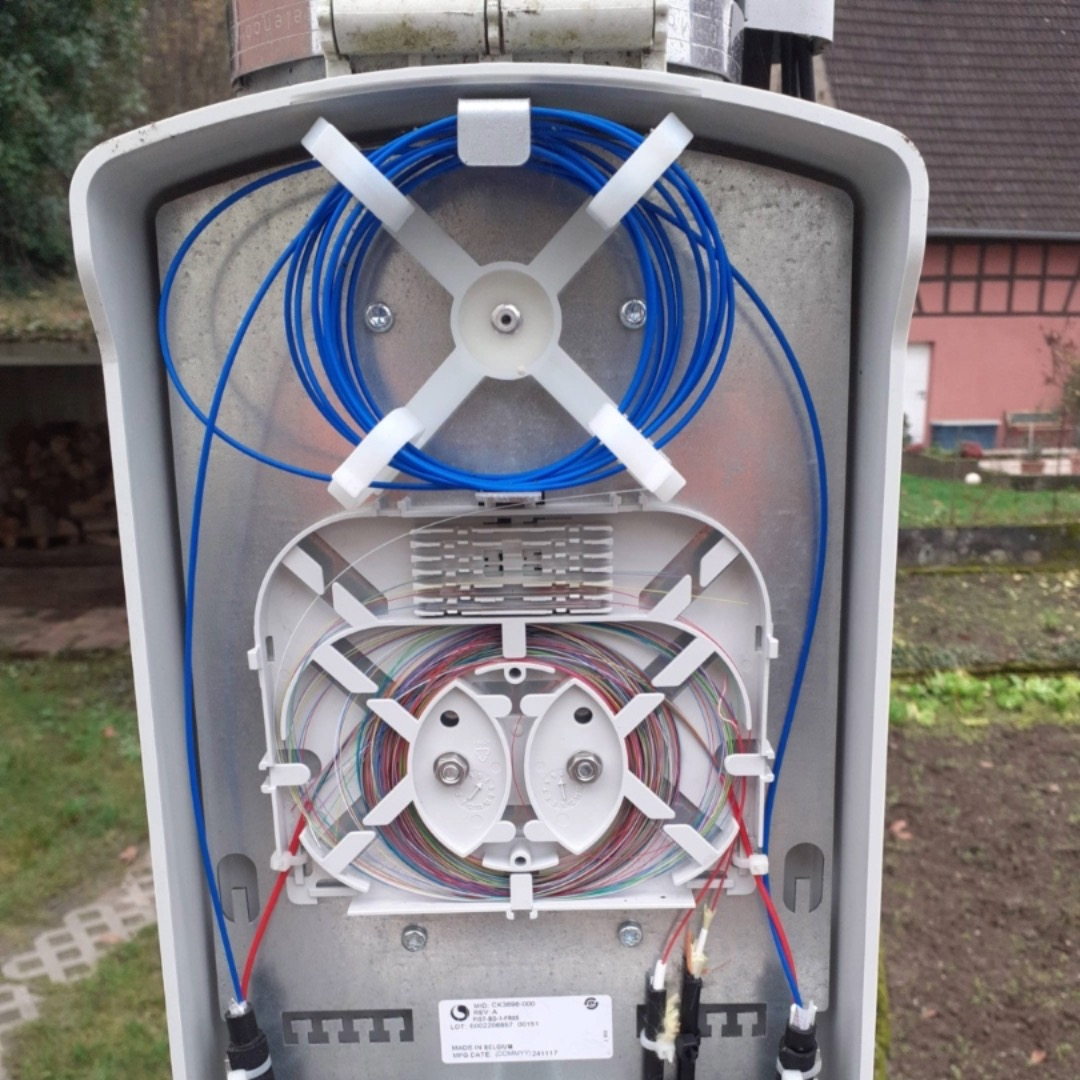
\includegraphics[width=\textwidth]{img/pbp.jpg}
      \caption{PB poteau}
    \end{minipage}
\end{figure}

Comme pour les points de branchement, il existe plusieurs 
types de points de mutualisation. Les plus courants 
sont les \gls{PMI} et les \gls{PMZ} du type que nous pouvons 
observer en image ci-dessous. Les PMI sont des points de mutualisation
immeubles, tandis que les PMZ sont des points de mutualisation
"de rue".\\
\begin{figure}[htbp]
    \centering
    \begin{minipage}[b]{0.4\textwidth}
		{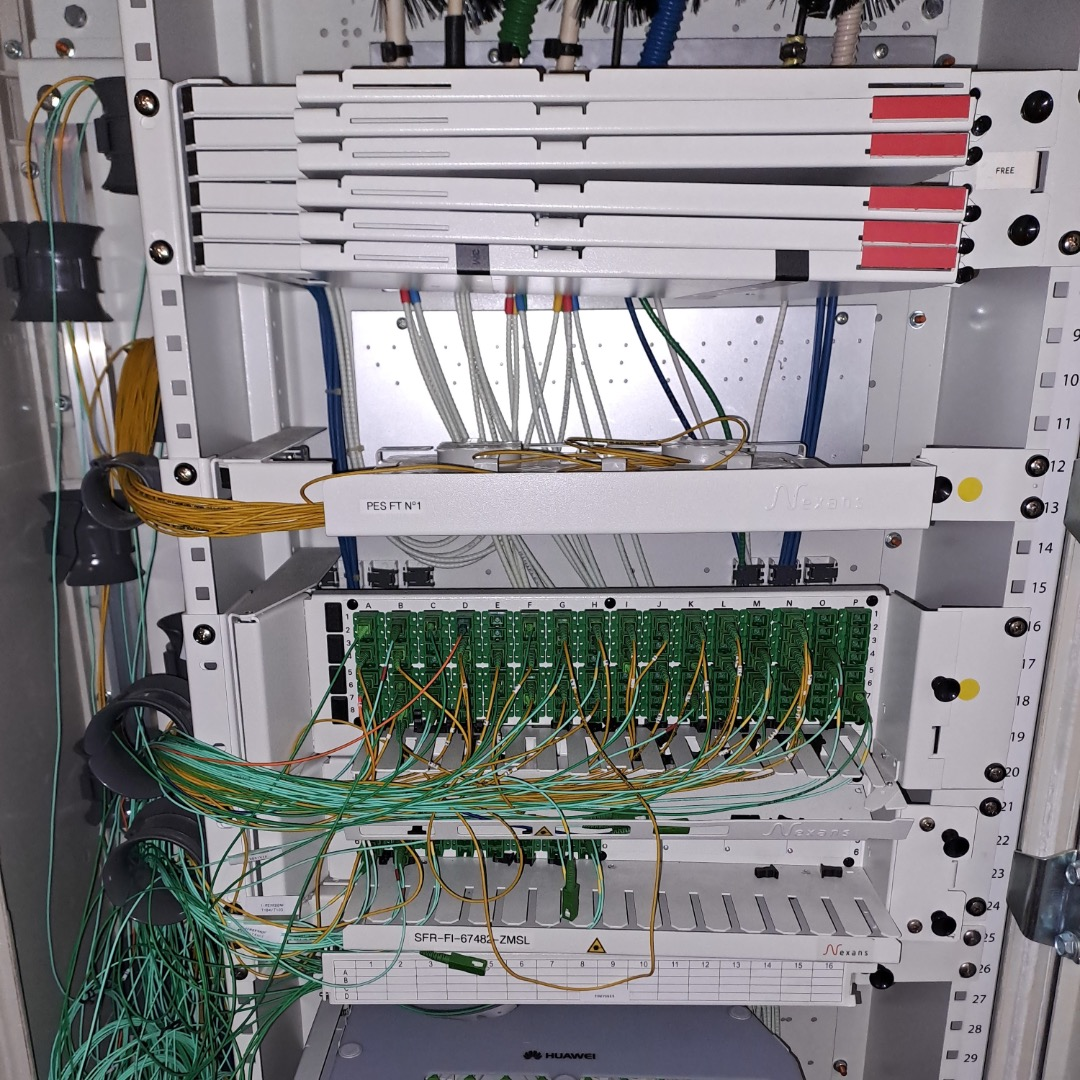
\includegraphics[width=\textwidth]{img/pmi.jpg}}
      \caption{PMI}
    \end{minipage}
    \hspace{0.5cm} % Espace horizontal entre les deux images
    \begin{minipage}[b]{0.4\textwidth}
      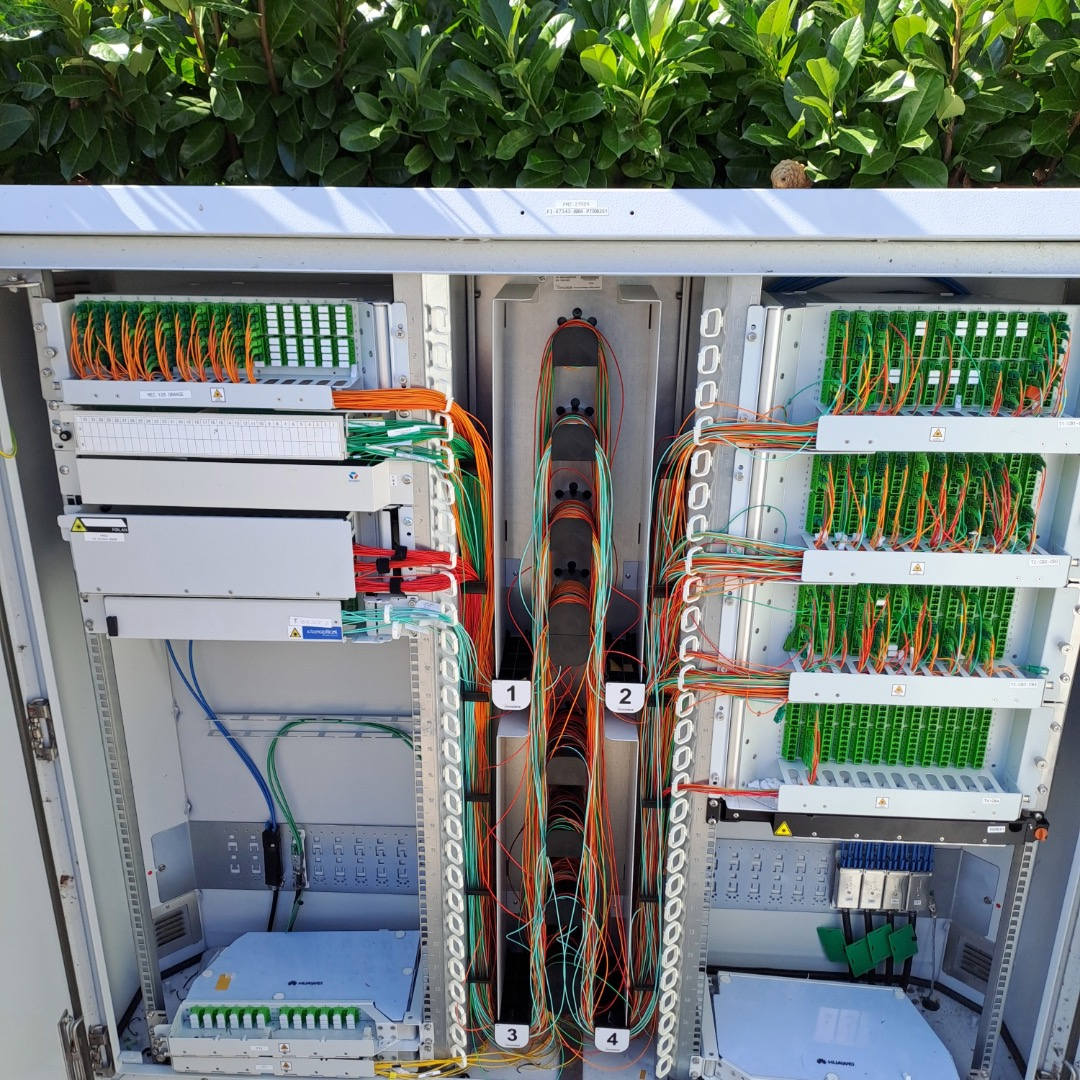
\includegraphics[width=\textwidth]{img/pmz.jpg}
      \caption{PMZ}
    \end{minipage}
\end{figure}

Lorsque les branchements au point de mutualisation (PM) ont été réalisés,
nous entamons l'installation des équipements. Nous commençons par mettre en place la Livebox,
un élément central de notre service.
Une fois que la Livebox est en place et fonctionnelle,
nous passons à l'installation des décodeurs. Ils
permettent à nos clients d'accéder à la télévision via la fibre optique
sans passer par un satellite. 
Après avoir installé les équipements Orange, nous assistons également
nos clients dans la connexion au Wi-Fi de leurs appareils personnels.

\newpage
Puis, pour garantir une couverture Wi-Fi optimale, nous utilisons une
application interne développée par Orange,
nommée APIE. Cette dernière nous permet d'effectuer
une analyse approfondie de la couverture Wi-Fi dans chaque pièce
de la résidence du client. Grâce à cette analyse,
nous sommes en mesure d'identifier les éventuelles zones
présentant une couverture Wi-Fi insuffisante. En conséquence,
nous pouvons prendre des mesures telles que
l'installation de répéteurs Wi-Fi avec l'accord du client 
pour étendre la portée du signal,
assurant ainsi une connectivité fiable dans l'ensemble de l'espace couvert.\\

Enfin, un compte rendu détaillé des mesures de couverture Wi-Fi
et généré par l'application APIE. Ce rapport détaillé est
ensuite envoyé au client par e-mail. Il offre au client une
vision claire et transparente de la qualité de la couverture Wi-Fi
de son domicile.
\subsubsection{Conclusion}
La plupart de ces installations se sont toujours 
bien déroulées. Les clients sont pour la majeure partie
du temps des personnes agées qui sont contents 
de voir qu'un "jeune" prenne le temps de leur 
expliquer la technologie. C'est d'autant plus 
satisfaisant pour moi car je me sens utile, et 
ça me fait plaisir de voir que je peux 
apporter un savoir qui semble si facile pour moi 
mais qui est si compliqué pour eux.\\

La seule fois où j'ai eu un problème, c'était
lorsque je suis arrivé chez une cliente qui était 
déjà sur les nerfs dès mon arrivé car elle avait
déjà eu plusieurs rendez-vous mais que personne 
ne lui avait installé la fibre (pour des problèmes
de continuité), alors que moi 
j'intervenais pour installer les équipements 
Orange, et non pour la fibre. Il s'agissait d'une erreur 
de notre côté car le rendez-vous avait mal 
été renseigné. J'ai alors fait face à une colère 
que je n'avais jamais encore rencontré dans le monde 
professionnel et j'ai du faire preuve de sang-froid. 
Mais même en étant calme, il était 
difficile de la raisonner et de lui faire comprendre 
que même si elle s'énervait, je ne pouvais rien faire
pour elle. Magré tout, j'ai réussi à la raisonner et
à lui expliquer la situation. Nous 
avons pu cette fois-ci planifier correctement 
le rendez-vous pour l'installation de la fibre.\\

Cette situation m'a permis de comprendre que 
finalement, peu importe la situation, il faut
toujours savoir garder son calme, et qu'avec les 
bons mots, on peut arriver à tout. Comme le disait 
si bien Hubert dans le film 
"La Haine" : \textbf{\textit{La haine attire la haine}}.

\newpage
\subsection{Les VQSE (Vérification Qualité Sécurité Environnement)}
\subsubsection{Explications}
Dans cette troisième section, nous allons
aborder un autre type de mission essentiel
au sein d'Orange : Les VQSE (Vérifications
Qualité, Sécurité et Environnement). 
Ces vérifications revêtent une
importance capitale, car elles visent
à garantir que chaque installation
fibre optique chez nos clients
particuliers faites par nos partenaires
soit réalisée avec le
plus haut niveau de qualité et de conformité.
Les VQSE se divisent en deux types de contrôles,
tous deux fondés sur une base commune :
l'inspection des installations
fibre chez nos clients.

\subsubsection{VQSE à froid}
Le premier type de contrôle VQSE,  "contrôle à froid,"
représente une étape essentielle dans notre
processus de vérification de la conformité de
nos installations fibre optique chez
les particuliers. Ce contrôle intervient
après les travaux d'installation et
s'appuie sur une série de procédures pour
garantir que chaque étape a été effectuée correctement.

L'un des aspects fondamentaux de ce
contrôle est de s'assurer que les positions
au point de mutualisation (PM) sont
respectées. Cela est important pour que notre sytème 
d'informations soit toujours à jour. Tout changement
doit être notifié dans le commentaire de relève 
ou suivi par l'appui à chaud lors d'une mutation.

L'étiquetage au point de branchement (PB) fait
également l'objet d'une vérification lorsqu'il
est possible de le faire. Chaque client au \gls{PB} doit
être étiqueté de manière précise et lisible,
garantissant ainsi une identification rapide
pour toute opération future de
maintenance ou de dépannage.

Un autre aspect du contrôle à froid
consiste à vérifier les photos prises
par nos techniciens partenaires avant/après
chaque étape de production fibre, en
particulier pour la Prise Terminale
Optique chez le client pour y vérifier
la présence du numéro de prise.  


\subsubsection{VQSE à chaud}
Le deuxième type de contrôle VQSE "contrôle à chaud,"
représente une étape proactive
dans notre démarche visant à garantir la qualité,
la sécurité et la conformité de nos installations
fibre optique chez les particuliers.
Contrairement au contrôle à froid, qui
intervient après l'exécution des travaux,
le contrôle à chaud se déroule directement
sur le site de production au moment où les
travaux ont lieu.

L'objectif de ce contrôle est
de s'assurer que les règles de sécurité
soient respectées lors de l'installation.
L'une des premières vérifications effectuées
concerne le balisage de la zone de travail.
Il est impératif que le technicien
responsable de l'installation délimite
de manière claire et appropriée la zone
où les travaux sont en cours. Cela garantit
la sécurité du personnel et des clients
potentiels présents dans les environs.
\newpage

Ci-après nous pouvons observer un exemple de balisage
correct à gauche, et incorrect à droite.
Nous constatons que le balisage à gauche est
clairement visible et approprié, tandis que 
sur l'image de droite, la chambre est ouverte
sans garde-fou ni cônes et qu'un passant pourrait 
malencontreusement tomber dans la chambre.\\
\begin{figure}[htbp]
    \centering
    \begin{minipage}[b]{0.4\textwidth}
		{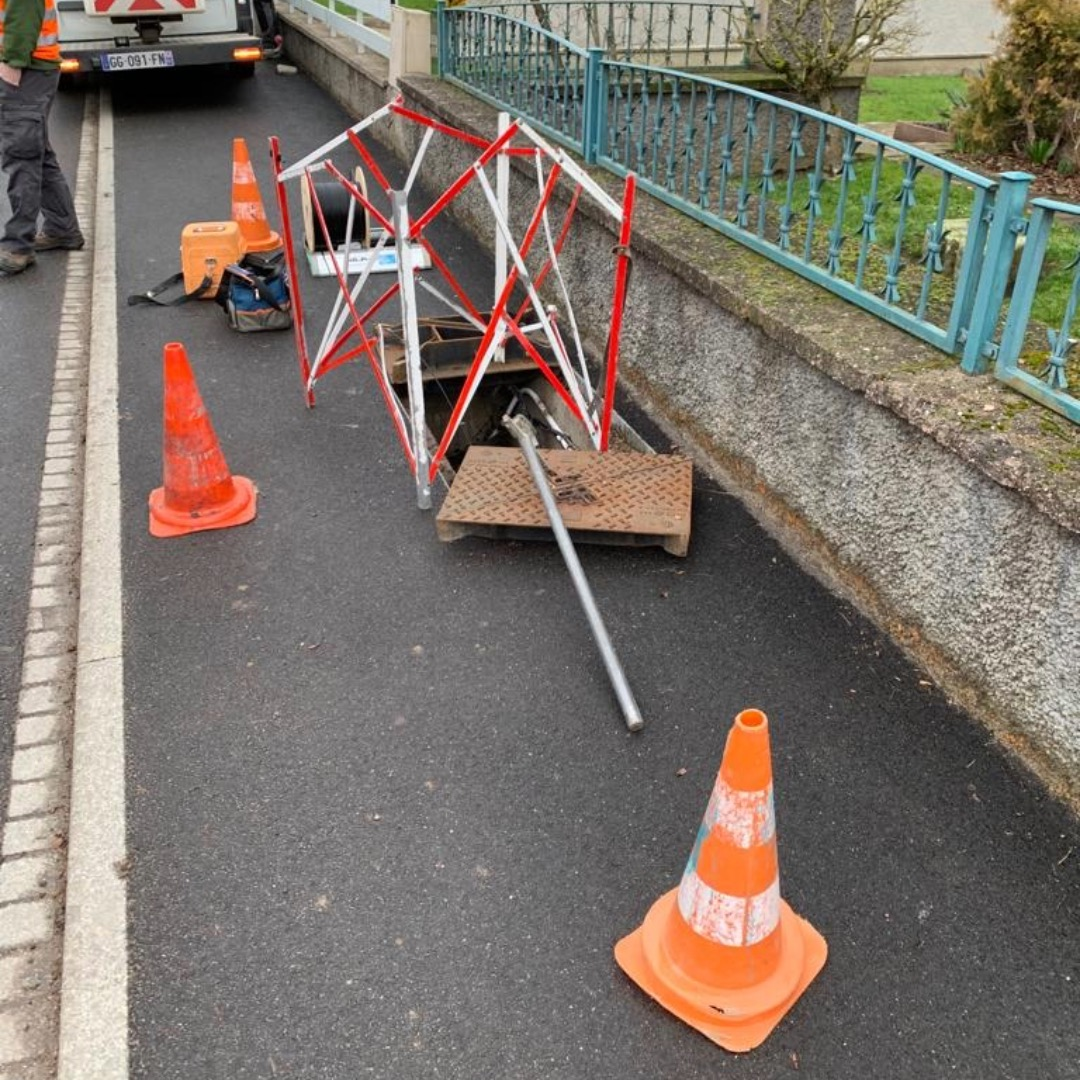
\includegraphics[width=\textwidth]{img/bok.jpg}}
      \caption{Balisage correct}
    \end{minipage}
    \hspace{0.5cm} % Espace horizontal entre les deux images
    \begin{minipage}[b]{0.4\textwidth}
      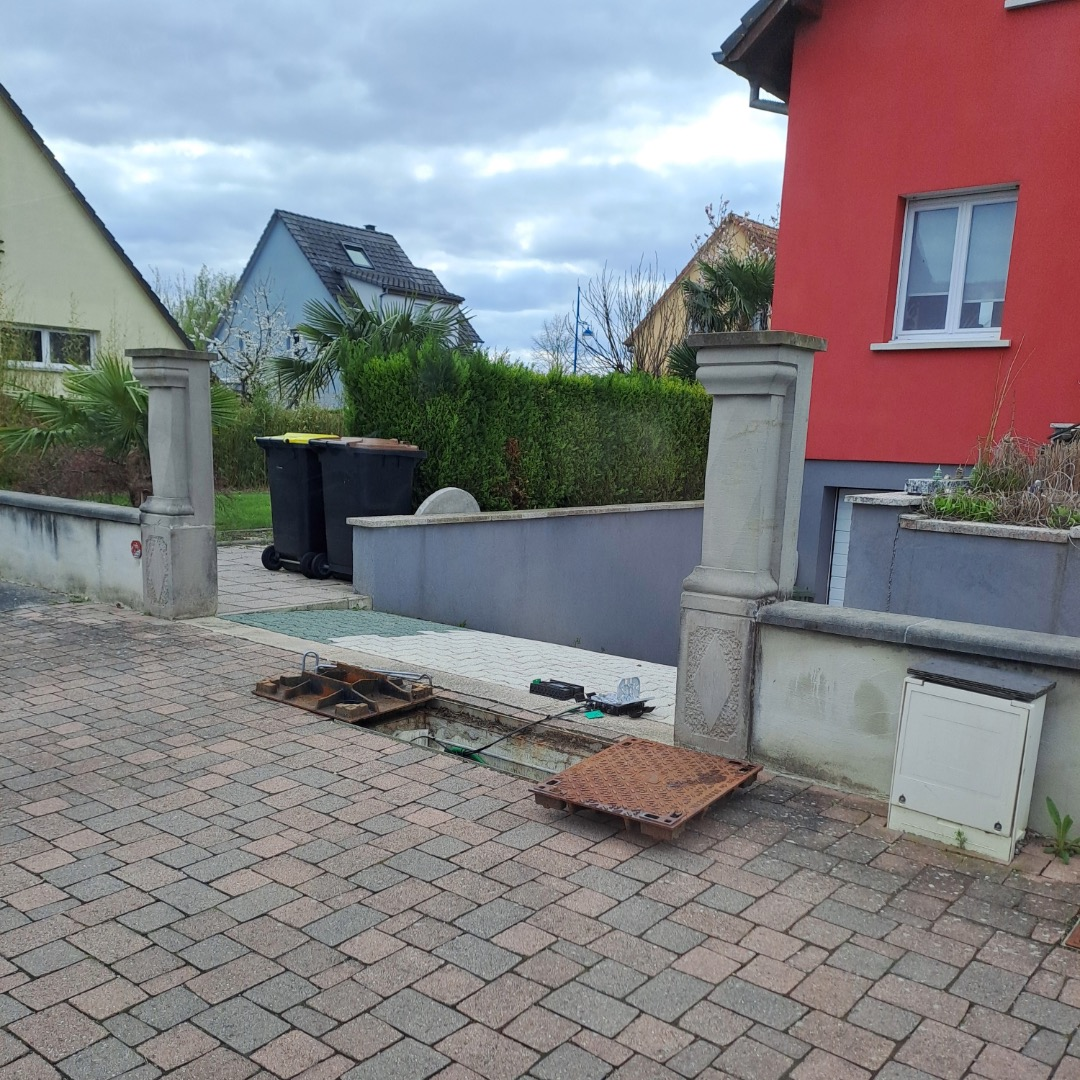
\includegraphics[width=\textwidth]{img/bpb.jpg}
      \caption{Balisage incorrect}
    \end{minipage}
\end{figure}

Un autre aspect important du contrôle à chaud est
de vérifier que le technicien dispose des
habilitations électriques nécessaires s'il
est amené à intervenir dans un tableau
électrique. Ces habilitations sont essentielles
pour garantir la sécurité électrique pendant
l'installation. Les techniciens doivent être
correctement formés et certifiés pour effectuer
des tâches spécifiques, ce qui réduit les
risques potentiels.\\

Le contrôle à chaud est également l'occasion
d'échanger avec les partenaires pour qu'ils 
puissent nous faire remonter les éventuels
problèmes récurrents qu'ils rencontrent sur le terrain, 
et ainsi pouvoir les remonter aux équipes concernées.\\

En somme, le contrôle à chaud comme à froid,
représente un engagement envers la sécurité et la qualité
dans notre processus d'installation. Il assure
que nos techniciens respectent strictement
les normes de sécurité et que la qualité de
l'installation répond à nos critères.
En cas de non-conformité, les entreprises 
partenaires ont alors des pénalités financières.
Ces types de contrôles sont essentiels pour garantir
que chaque installation est
effectuée en toute sécurité et avec la plus
haute qualité, tout en renforçant la confiance
de nos clients.


\newpage
\subsection{Les dépannages}
Alors que nous avons passé en revue les processus d'installation et
de contrôle qui constituent les fondements de nos services \gls{FTTH},
il est tout aussi essentiel d'explorer l'autre
facette de notre engagement envers nos clients : les dépannages.
En effet, même avec des installations de haute qualité et des
contrôles rigoureux, des pannes peuvent parfois survenir.
Dans cette section, nous aborderons en détail
les différents types de dépannages \gls{FTTH} afin de garantir une expérience sans
faille à nos clients.\\

Je procède à deux types de dépannages : les dépannages fibre pour les 
clients particuliers, et les dépannages d'une ancienne offre de téléphonie 
d'Orange : \gls{OPO}. Ce qui est pratique c'est que nous 
avons des outils de pré-diagnostique qui nous permettent de faire des tests
à distance et de savoir à l'avance où le problème pourrait se situer.

\subsubsection{Mon process de dépannage fibre}
Chaque technicien a sa propre manière de travailler mais tout en 
suivant le mode opératoire fournit par Orange. Pour ma part, 
lorsque j'ai un dépannage à faire, si je n'ai pas d'infos en commentaires,
j'appelle toujours le client. Je lui demande alors comment s'est-il
rendu compte de la panne, l'heure et le jour à laquelle il a 
constaté le problème. Je lui demande également s'il n'a pas fait de travaux
ou déplacé des meubles récemment. Si la panne est survenue après
des travaux, il est fort probable que le client ait sectionné la fibre.
Dans ce cas, je me rends chez le client pour tenter de ressouder si possible, 
ou alors si le problème se situe
en \gls{D2}
j'appelle Orange pour qu'ils s'occupent de faire intervenir l'opérateur
d'infrastructure.\\

Si le client au téléphone déclare ne pas avoir
effectué d'actions particulières, je me dirige
vers le point de mutualisation pour effectuer
une mesure à l'aide du JDSU OLP.\\

\begin{figure}[h]
	\centering
	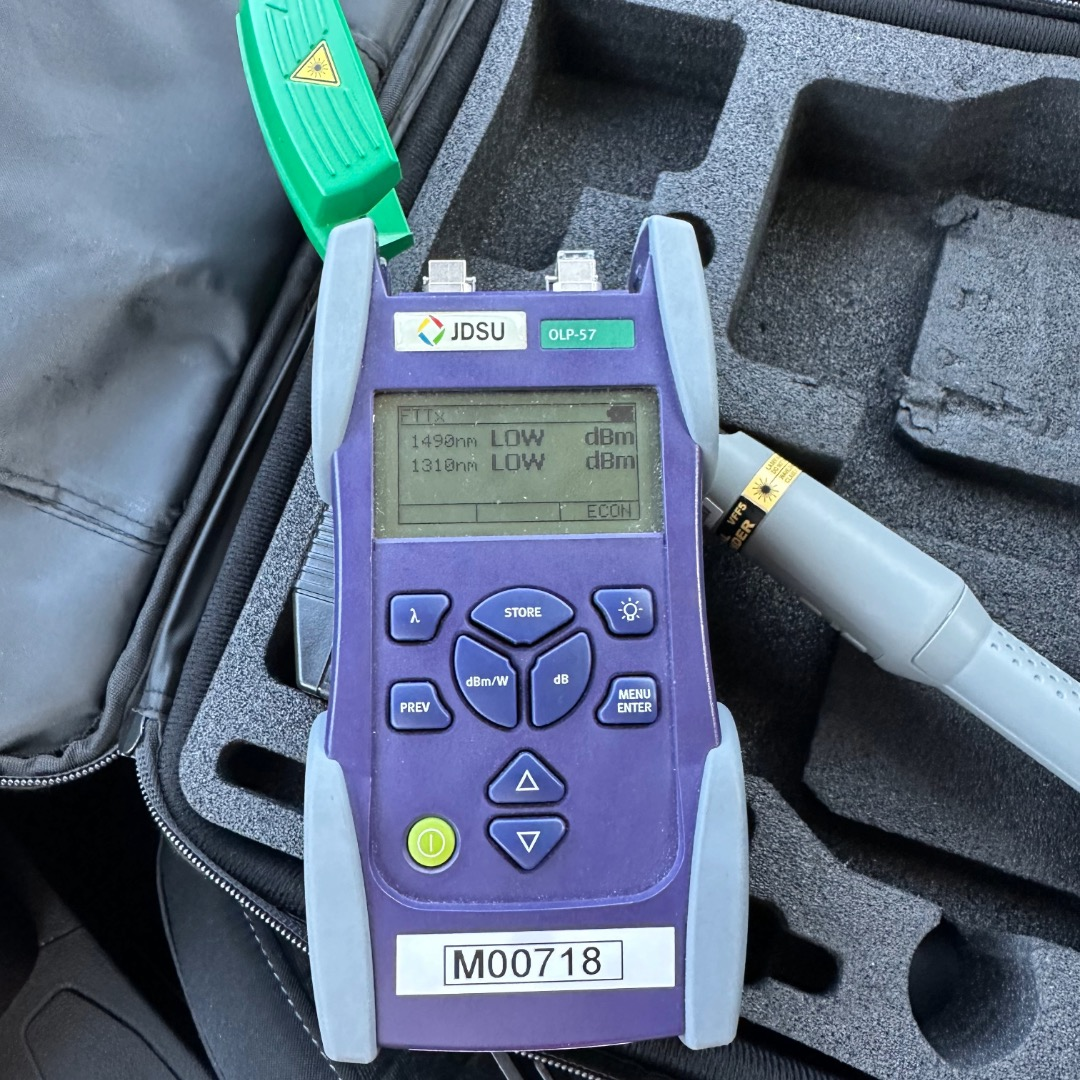
\includegraphics[scale=0.2]{img/olp.jpg}
	\caption{JDSU OLP}
\end{figure}

Cet appareil
permet de quantifier l'atténuation du signal
entre l'OLT et le PM. Lorsque la mesure affiche
une valeur aux alentours de -18 dBm, nous pouvons
conclure que le problème réside entre le \gls{PM} et
le client, excluant ainsi tout dysfonctionnement
du coupleur au PM. En principe nous pouvons savoir 
s'il y a un problème de coupleur ou de cable de transport 
en fonction de résultats de tests que nous faisons. Si nous 
voyons qu'aux mêmes heures, plusieurs pannes ont lieu sur
le même coupleur, nous pouvons alors en déduire que le problème
vient du coupleur ou du câble de transport.\\

Ensuite, je branche mon laser sur la position du client au
\gls{PM} et me rends au point de branchement
pour vérifier la présence de la lumière
du laser. Si elle est absente, cela indique
un problème situé entre le \gls{PM} et le \gls{PB}.
Si, au contraire, la lumière est visible,
je me rends chez le client pour vérifier
la présence de la lumière à son niveau.
Si la lumière n'est pas perceptible chez le
client, cela signifie que le problème se
situe entre le \gls{PB} et le client. En revanche,
si la lumière est visible chez le client,
je procède au rebranchement de la jarretière
optique du \gls{PM} et j'effectue une mesure à l'OLP
depuis la \gls{PTO} du client. En suivant ces étapes
méthodiques, il devient généralement possible
de diagnostiquer l'origine du problème de
manière efficace.

\newpage
\subsubsection{Les SAV OPO}
Découvrons maintenant le \gls{SAV} \gls{OPO}, l'ancienne offre de
téléphonie d'Orange qui, bien que moins sophistiquée
que Connect Pro, a joué un rôle essentiel dans nos offres
de téléphonie. L'offre est toujours en service pour les clients
qui l'ont souscrite avant l'arrivée de Connect Pro. Et donc, 
nous avons toujours des interventions à faire sur cette offre.\\

Parmi les défis majeurs auxquels les utilisateurs de l'Offre de
Téléphonie \gls{OPO} ont été confrontés, les soucis de communications
blanches se sont avérés être l'une des préoccupations les plus
récurrentes. Ces dernières se traduisent par des 
coupures inattendues ou une qualité de communication
altérée. Ces problèmes peuvent être frustrants, mais ils sont
souvent causés par deux raisons principales.\\

La première raison réside dans un problème de surcharge du
processeur de la Livebox, l'équipement central de notre offre
de téléphonie. Lorsque le processeur de la Livebox est surchargé,
il peut avoir du mal à gérer efficacement les appels, ce qui se
traduit par des interruptions ou une qualité audio médiocre.\\

La deuxième source de soucis de communications blanches est
liée aux boîtiers ATA (Adaptateur Téléphonique Analogique).
Ces boîtiers sont responsables de la conversion du signal
téléphonique analogique en signal numérique, permettant ainsi
aux téléphones traditionnels de fonctionner sur la technologie
numérique. Cependant, des problèmes techniques dans ces boîtiers
ATA pouvent entraîner des dysfonctionnements de la communication,
notamment des coupures ou des interférences.\\

Pour remédier à ces problèmes, la première chose à faire est 
de vérifier les branchements du client et 
en général nous nous rendons compte qu'il y a d'anciens 
boitiers ATA qui ne sont plus essentiels, alors nous 
les enlevons. Ensuite, nous
nous connectons sur l'interface d'administration de la livebox 
pour vérifier s'il ne manque pas une mise à jour ou si le 
processeur n'est pas surchargé. Si toutefois, nous 
ne parvenons pas à nous connecter à la box, nous pouvons 
toujours appeler Orange pour qu'ils puissent rentrer 
à distance en lignes de commandes pour 
vérifier si des problèmes sont présents.
Au terme de ces vérifications, il fallait souvent 
faire une mise à jour ou le remplacement de la Livebox, 
ce qui résolvait la grande majorité des problèmes.\\

Les soucis de communications blanches dans l'Offre de Téléphonie
\gls{OPO} sont gérés avec succès grâce à notre engagement à résoudre
les problèmes techniques pour garantir une expérience client
optimale. De plus, nous informons nos clients que ces problèmes peuvent
être complètement éliminés en optant pour l'offre Connect Pro,
une solution de téléphonie plus avancée, sans avoir une
augmentation tarifaire significative. Cette transition vers
Connect Pro offre une expérience de communication plus stable,
tout en démontrant notre engagement continu à fournir des
services de téléphonie de qualité et adaptés aux besoins
changeants de nos clients.

\newpage
\subsection{Les expertises}
L'expertise, dans le cadre de nos interventions en télécommunications,
représente une étape avancée du processus de résolution de problèmes.
Cette démarche survient généralement en dernier recours, après que
plusieurs interventions de Service Après-Vente (SAV) n'aient pas
réussi à résoudre les problèmes rencontrés par le client. Le cheminement
typique est le suivant : \gls{PMS}, \gls{ROI} puis \gls{EXP}.\\

Lorsque nous entamons une expertise, nous nous rendons généralement
sur place en compagnie de l'Opérateur d'Infrastructure (OI) qui gère
la zone d'intervention. L'objectif de l'expertise est de trouver
une solution définitive au problème du client, de sorte qu'aucune
autre intervention ne soit nécessaire. Dans certains cas, le problème
peut être résolu dès la première visite, mais il arrive que des
techniciens partenaires ne parviennent pas à effectuer le travail de
manière optimale, ce qui peut entraîner le renvoi du dossier pour
des niveaux de service supérieurs, passant ainsi par les étapes de
PMS, ROI, et enfin EXP.\\

L'expertise est souvent nécessaire lorsque la situation est complexe
ou qu'il est essentiel de collaborer avec l'Opérateur
d'Infrastructure pour rétablir la connexion du client. Notre objectif
lors de l'expertise est de garantir que tous les services du client
sont rétablis et opérationnels, tout en veillant à ce qu'aucun
autre problème ne subsiste. 

\newpage
\subsection{Ma mission chez Wrigley}
\subsubsection{Mise en contexte}
En mai 2023, j'ai eu l'opportunité d'effectuer une mission
ponctuelle chez Wrigley grâce à l'initiative de mon manager au
sein de l'équipe entreprise du 68. À ce moment-là, l'équipe faisait
face à un sous-effectif et était confrontée à la tâche de remplacer
une vingtaine de switchs dans l'entreprise. Mon manager m'a
contacté pour me proposer cette opportunité, avec l'intention de
me permettre d'acquérir une expérience nouvelle et d'aussi
pouvoir aider aussi les collègues du 68. Cette mission
s'est révélée être une occasion enrichissante de mettre en pratique
mes compétences et d'explorer un domaine différent de mon travail habituel.

\subsubsection{Objectif}
L'objectif de cette mission était
de remplacer une vingtaine de switchs
Cisco dans toutes les baies de brassage de l'entreprise.
Dans certains cas, il fallait
réduire le nombre de switchs, tandis que dans d'autres, il
était nécessaire d'augmenter leur nombre pour optimiser
l'infrastructure réseau de Wrigley.

La mission a duré quatre jours, au cours desquels 
mon collègue Alain et moi-même étions responsables 
de réaliser l'installation physique
du matériel, notamment le remplacement des switchs existants.
Une fois le matériel en place, une étape cruciale de la mission
était de connecter notre PC en utilisant une connexion série au
switch nouvellement installé. Cette connexion nous
permettait de mettre en place une interface de communication
avec les ingénieurs d'\gls{OB},
qui étaient situés à distance.
Grâce à cette connexion, les ingénieurs pouvaient alors prendre
la main de notre PC et injecter
la configuration spécifique des switchs de manière à les adapter
aux besoins et aux exigences de l'entreprise.
Une fois la configuration injectée, nous devions alors brasser 
les câbles des différents postes de travail sur les nouveaux switchs
en fonction des positions qui nous étaient indiquées par les
ingénieurs ayant fait la configuration.

\subsubsection{Déroulement}
Le déroulement de la mission était organisé de manière à optimiser
notre efficacité tout en minimisant les interruptions. Avec une
dizaine de salles où nous devions intervenir, nous avons mis en place une stratégie
bien coordonnée pour maximiser notre productivité. Pendant que je
prenais en charge le matériel nécessaire pour une salle donnée,
j'installais les nouveaux switchs dans les baies de brassage
correspondantes. Pendant ce temps, mon collègue Alain se chargeait
de connecter son PC aux switchs fraîchement installés, permettant
ainsi aux ingénieurs de procéder à la configuration à distance.

L'un des aspects clés de notre approche était de maintenir un
rythme fluide. Pour ce faire, j'anticipais généralement en ayant
une à deux salles d'avance. Cela signifiait
que dès qu'une salle était terminée, nous pouvions immédiatement
passer à la suivante, minimisant ainsi toute perte de temps entre
les installations. Pour me guider dans l'entreprise Wrigley et
m'assurer de trouver rapidement chaque salle, j'étais accompagné
par un membre du personnel de Wrigley qui connaissait bien les locaux.
Cette collaboration efficace nous a permis de mener à bien la mission
de manière organisée et efficiente.

\subsubsection{Corrélations avec le B.U.T.}
Au cours de ma mission, j'ai eu l'opportunité de mettre en
pratique les compétences acquises lors de ma formation au B.U.T.
L'une des facettes les plus marquantes de cette expérience a
été ma capacité à comprendre et à interagir avec les ingénieurs
d'\gls{OB} chargés de configurer les nouveaux switchs Cisco.

En effet, lors de la configuration à distance des switchs,
j'ai pu identifier et reconnaître des commandes que j'avais
précédemment étudiées à l'IUT. Cela signifie que lorsque les
ingénieurs d'OB ont commencé à entrer des commandes pour
configurer les switchs, j'ai pu suivre et comprendre le processus,
car il s'agissait souvent des mêmes commandes que j'avais apprises à
l'IUT. Cette corrélation entre ce que j'avais appris et ce que
je voyais en action sur le terrain m'a permis d'avoir une
compréhension approfondie de la configuration des switchs Cisco.
Par exemple, lorsqu'ils ont configuré les ports VLAN
pour segmenter le réseau ou encore quand ils ont 
configuré les ports en mode trunk pour permettre
la communication entre les switchs tout en 
transportant le trafic de plusieurs VLAN.\\

\newpage
\section{Conclusion}
Mon parcours d'alternance chez Orange a été rythmé par des missions
significatives qui m'ont permis de me familiariser avec les solutions
de téléphonie IP. J'ai participé à
l'implémentation de l'offre Connect pro, spécialement conçue pour
répondre aux besoins des petites entreprises, sans nécessiter
l'installation d'un serveur sur place. J'ai également
contribué à des prestations d'installation experte, garantissant
l'intégration efficace du matériel chez le client et la configuration
optimale du réseau pour une connectivité sans faille. Les contrôles
à chaud et à froid effectués ont été essentiels pour maintenir un
haut niveau de qualité de service, tout en respectant les normes
strictes de sécurité et d'environnement. J'ai aussi participé
aux services après-vente fibre optique et des offres
OPO, où j'ai pu mettre en pratique mes
compétences techniques et d'analyse pour résoudre les problèmes.\\

Ma formation reçue chez Orange a été un pilier fondamental de mon
développement professionnel. Elle m'a doté des outils nécessaires
pour une transition en douceur vers un travail autonome et responsable.
Les interactions avec mon formateur, toujours à l'écoute, ont enrichi
mon expérience et renforcé ma confiance en mes capacités. Les défis
rencontrés, notamment lors d'installations 
dans des environnements complexes tels que de grands restaurants,
ont aiguisé mes compétences d'analyse et ma capacité à gérer l'imprévu.
La réalisation d'une maquette explicative pour accompagner les clients
dans la configuration de leurs services a été une occasion de démontrer
mon engagement envers la satisfaction client et d'innover dans la
communication. Sur le plan personnel, cette alternance a
été une période d'intégration et de collaboration au sein d'une équipe
dynamique, me permettant de mieux comprendre le fonctionnement interne
d'une grande entreprise.\\

Pour conclure, mon objectif est de devenir ingénieur avant-vente,
une aspiration que cette alternance chez Orange a contribué à solidifier.
L'expérience acquise, tant sur le plan technique que sur le plan des valeurs
de l'entreprise, m'a préparé à relever les défis à venir. Les compétences
techniques approfondies que j'ai développées sont le fondement sur lequel
je souhaite bâtir ma carrière. Je suis résolu à continuer à apprendre et à
me perfectionner, en portant avec moi les leçons apprises et les succès
obtenus pendant cette période formatrice. Mon ambition est de contribuer
avec innovation et efficacité aux solutions avant-vente d'Orange, en
apportant ma vision et mon expertise technique au service de la stratégie
de l'entreprise.
\newpage
\pagestyle{empty}
\appendix
\part{\Large{Annexes}}
\newpage
\parttoc 


\newpage
\pagestyle{fancy}
\glsaddall

\section{Glossaire}
\begingroup
\renewcommand{\addcontentsline}[3]{}
\printglossary[type=\acronymtype, title=Acronymes]
\endgroup

\newpage
\section{Bibliographie}
\bibliographystyle{elsarticle-num}
\bibliography{rapport.bib}

\newpage
\section{Images}
\begin{figure}[h]
	\centering
	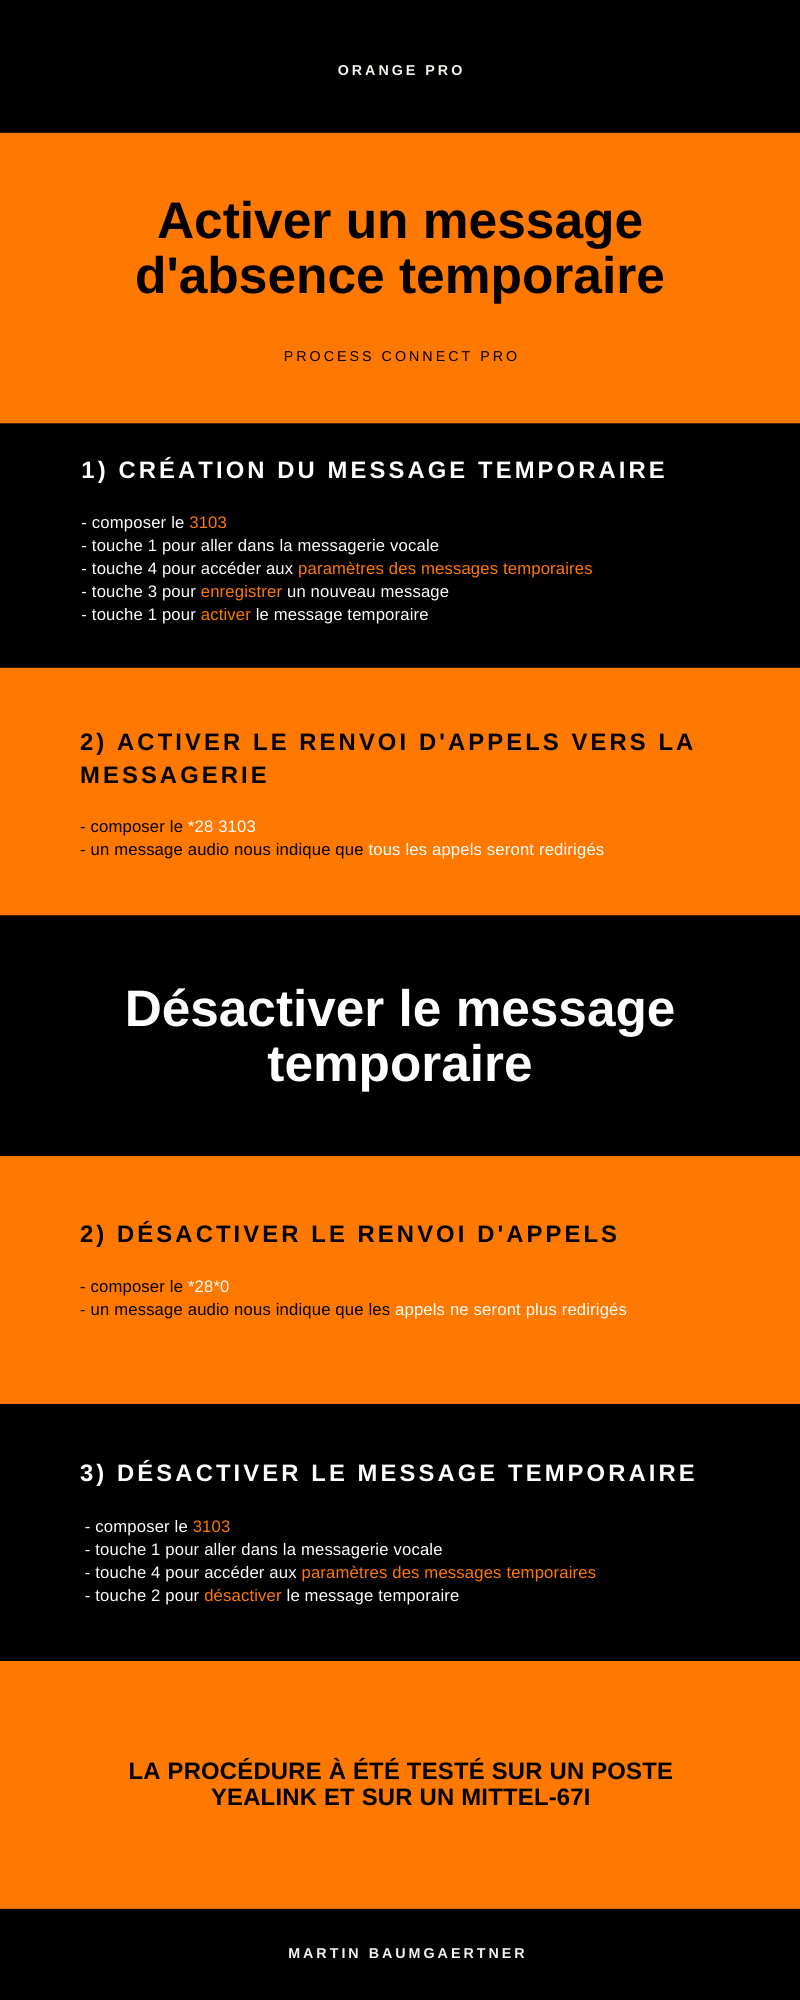
\includegraphics[width=0.45\textwidth]{img/maquette.png}
	\caption{Maquette explicative}
\end{figure}

\end{document}

